\documentclass[conference,10pt]{IEEEtran}
\usepackage[T1]{fontenc}
\usepackage{amsmath,amssymb,amsthm}
\usepackage{graphicx,booktabs,multirow}
\usepackage{cite}
\usepackage[hidelinks]{hyperref}
\hypersetup{pdftitle={Learning Energy-Efficient Uplink Access with Asynchronous Packet Deadlines},pdfauthor={}}
\newtheorem{proposition}{Proposition}
\newcommand{\E}{\mathbb{E}}
\newcommand{\ind}{\mathbf{1}}
\newcommand{\OFF}{\mathsf{OFF}}
\newcommand{\clip}{\operatorname{clip}}
\newcommand{\SavingFour}{-0.7}
\newcommand{\EnergyFour}{1.007}
\newcommand{\FeasibleFour}{0.993}
\newcommand{\PowerFour}{3.85}
\newcommand{\SavingSix}{36.6}
\newcommand{\EnergySix}{1.094}
\newcommand{\FeasibleSix}{0.986}
\newcommand{\PowerSix}{4.36}
\newcommand{\SavingEight}{56.7}
\newcommand{\EnergyEight}{1.213}
\newcommand{\FeasibleEight}{0.994}
\newcommand{\PowerEight}{5.30}
\newcommand{\SavingTwelve}{70.5}
\newcommand{\EnergyTwelve}{1.623}
\newcommand{\FeasibleTwelve}{0.984}
\newcommand{\PowerTwelve}{8.87}
\newcommand{\ConfirmEnergy}{1.217}
\newcommand{\ConfirmFeasible}{0.993}
\newcommand{\ConfirmSacEnergy}{3.028}
\newcommand{\ConfirmSavingSac}{59.8}
\newcommand{\ConfirmSavingPaced}{56.9}
\newcommand{\ConfirmGapSac}{1.811 [1.648, 1.999]}
\newcommand{\ConfirmGapVOne}{4.073 [2.838, 5.634]}
\newcommand{\ConfirmGapVSparse}{4.459 [2.689, 5.737]}


\title{Learning Energy-Efficient Uplink Access\\with Asynchronous Packet Deadlines}
% Replace this draft placeholder with the complete author list before submission.
% ICC 2027 requires the PDF author list and title to match the EDAS record.
\author{\IEEEauthorblockN{Author information to be supplied}}

\begin{document}
\bstctlcite{bibcontrol}
\maketitle
\begin{abstract}
Periodic devices can save transmit energy by spreading service over several
slots, but overlapping transmissions can erase this benefit in shared uplinks.
We study distributed subchannel, power, and silence decisions for asynchronous
periodic packets under per-device deadline requirements. Devices use local
packet state, delayed public received-power measurements, and private service
feedback. A shared recurrent policy is trained using multi-agent proximal
policy optimization and compared with calibrated local rules and centralized
zero-loss references. Across 200 held-out instances per network size, three
training seeds, and two executions per instance, the fixed-penalty policy
reduces mean normalized transmit energy by \SavingSix\%, \SavingEight\%,
and \SavingTwelve\% relative to the strongest evaluated feasible local rule
for 6, 8, and 12 devices sharing four subchannels. Its feasible-episode
fraction is at least 0.984. With four devices, energy is about 0.7\% above
the exact zero-loss reference. On a separate 200-instance confirmation set
with eight devices, energy is \ConfirmSavingSac\% lower than an XR-SBPC-style
discrete soft actor--critic adaptation using the same energy reward and
execution information. The learned policy combines low-power transmission
with selective silence and exhibits lower co-channel overlap and interference
loss. These results demonstrate the energy benefits of learned distributed
access for asynchronous periodic traffic.
\end{abstract}

\begin{IEEEkeywords}
distributed access, periodic traffic, deadline constraints, power control,
multi-agent reinforcement learning
\end{IEEEkeywords}

\section{Introduction}
Periodic sensing and control traffic poses an energy--reliability tradeoff in
shared uplinks. A device can lower its transmit power and accumulate service
across several slots before its deadline. However, extending transmission also
increases the opportunities to interfere with other devices. With heterogeneous
periods and unaligned arrival phases, independently choosing a low power does
not ensure low network energy. Devices must also learn when to transmit and
which subchannel to use, including when to remain silent despite a pending
packet.

The energy benefit of stretching a transmission under deadline constraints is
established by classical packet-scheduling results~\cite{lazy2002}. In a shared
uplink, the practical question is how much of this benefit a distributed
controller can retain using delayed local feedback. High packet delivery alone
does not answer this question: frequent maximum-power transmissions may be
reliable but expensive. Conversely, low energy can result from leaving
difficult devices unserved. A useful evaluation must therefore combine
per-device reliability checks, an energy-aware local baseline, and an explicit
centralized reference.

Learning-based distributed spectrum access has been studied using recurrent
policies with local acknowledgments~\cite{naparstek2019}. Joint subband and
power decisions for delivering a payload within a time budget appear in
vehicular multi-agent reinforcement learning (MARL)~\cite{liang2019}.
For periodic mission-critical traffic, reinforcement-learning power control
has also been developed for reliability-constrained single-link
transmission~\cite{guo2023}. More recently, recurrent MARL has addressed spectrum
and power allocation with stochastic traffic in multicell
networks~\cite{zhang2025}. These works establish that neither joint resource
selection nor recurrent MARL is by itself a new contribution.

The particularly close XR-SBPC study~\cite{bagherinejad2025} combines periodic
traffic with offsets, accumulated Shannon service, and discrete subband--power
actions, including silence. It addresses reliability in a network of downlink
subnetworks and uses observations that include neighboring actions and current
link gains. Our study instead examines transmit-energy minimization under
per-device delivery requirements in a common-receiver uplink. Execution uses
only the device's own history and AP feedback, without access to other devices'
actions, queues, or phases. We evaluate this information model against
centralized references computed for the same packets and discrete power menu.

We instantiate a shared, subchannel-equivariant recurrent policy within
multi-agent proximal policy optimization (MAPPO)~\cite{yu2022}, and compare a
fixed violation penalty with local dual adaptation inspired by
state-augmented constrained reinforcement learning~\cite{calvo2021}.
The contribution is an evaluated access-control formulation and benchmark,
with three concrete components:
\begin{enumerate}
\item We specify asynchronous periodic delivery with accumulated service,
      joint subchannel--power--silence actions, and an explicit causal
      information boundary for decentralized execution.
\item We construct discrete-power zero-loss energy references: an exact
      interference-free solution when devices do not outnumber subchannels,
      and a separable lower reference plus a feasible cyclic orthogonal
      schedule at higher loads.
\item We quantify held-out energy and reliability with multiple training
      seeds, calibrated local rules, and paired uncertainty estimates.
      Additional diagnostics identify reduced transmission overlap as an
      observed correlate of the gains and expose the cost of insufficient
      training and residual per-device failures.
\end{enumerate}
Our conclusions concern static, frequency-flat channels and transmit energy.
They establish neither a general constraint guarantee for MAPPO nor superiority
over all available learning algorithms.

\section{System Model and Control Objective}\label{sec:model}
\begin{figure}[t]
\centering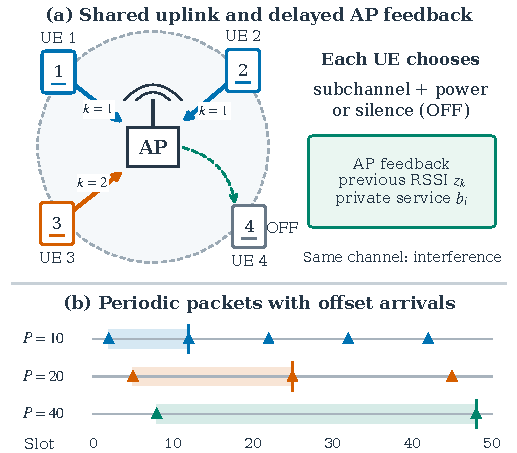
\includegraphics[width=\columnwidth]{figures/system_scenario.pdf}
\caption{Periodic uplink access. Solid arrows illustrate transmissions;
UEs 1 and 2 reuse a subchannel and interfere at the AP. Dashed feedback is
received even during silence. Shading marks the first packet window in each
illustrative traffic class; triangles denote arrivals and vertical bars its
deadline. Physical slots are synchronized, while arrival phases differ.}
\label{fig:scenario}
\end{figure}
\subsection{Periodic uplink and accumulated service}
Figure~\ref{fig:scenario} illustrates an access point (AP) receiving uplink
packets from $N$ devices over $K$
orthogonal subchannels. Slots have duration $\tau$, and each subchannel has
bandwidth $B$. Device $i$ generates a packet of $L_i$ bits at
$a_{i,m}=\varphi_i+mP_i$, with deadline $d_{i,m}=a_{i,m}+P_i$.
The phase $\varphi_i$ is drawn independently and uniformly from
$\{0,\ldots,P_i-1\}$. Physical slots are synchronized; asynchronous traffic
refers to the packet-arrival phases. At most one packet is pending per device.

In slot $t$, device $i$ selects $a_i(t)\in\{\OFF\}\cup
(\{1,\ldots,K\}\times\mathcal P)$, where $\mathcal P$ is the positive
discrete-power menu. Let $k_i(t)$ and $p_i(t)$ denote its chosen subchannel and
power, with $p_i(t)=0$ for $\OFF$. The noise power per subchannel is $\sigma^2$.
The AP decodes each device's signal by treating interference as noise.
For an active device,
\begin{align}
\gamma_i(t)&=\frac{p_i(t)g_i}
 {\sigma^2+\sum_{j\ne i:k_j(t)=k_i(t)}p_j(t)g_j},\label{eq:sinr}\\
b_i(t)&=\tau B\log_2(1+\gamma_i(t)),\qquad e_i(t)=\tau p_i(t).
\label{eq:service}
\end{align}
The gain $g_i$ is static and identical across subchannels within an instance;
subchannel selection controls co-channel interference.
For silence, $b_i(t)=e_i(t)=0$.

We use an ideal accumulated-mutual-information model, motivated by incremental
redundancy hybrid ARQ~\cite{caire2001}. A packet completes once the sum of its
slot services reaches $L_i$. Even if its final transmission
provides excess service, a device occupies and pays for the whole slot. At each
slot boundary, the environment first applies service, then settles expiring
packets, and finally releases new packets. Unfinished bits are discarded at
expiry. A device without a pending packet must select $\OFF$ but continues
receiving observations. We measure radiated transmit energy using
\eqref{eq:service}.

\subsection{Causal execution information}
At a slot's start, device $i$ knows its remaining bits $s_i(t)$, remaining time
$D_i(t)$, its packet size and period, and its preceding action and outcome.
The AP supplies the previous slot's per-subchannel received power $z_k(t-1)$,
including noise, and the device's private service feedback $b_i(t-1)$.
It supplies no scheduling decision. Devices do not exchange messages, and the
policy receives no device identifier, global slot index, topology, or other
devices' queues, phases, gains, and actions.

These observations contain useful channel information. After transmitting at
power $p$ on subchannel $k$, a device can infer
\begin{equation}
\widehat\gamma=2^{b/(\tau B)}-1,\qquad
\widehat I=\frac{z_k}{1+\widehat\gamma},\qquad
\widehat g_i=\frac{z_k-\widehat I}{p}.\label{eq:estimate}
\end{equation}
The gain estimate is retained across packets. Exact feedback and a static
channel make this estimate exact after a transmission in the ideal model;
the remaining uncertainty includes other devices' future actions. All
distributed baselines use the same permitted observation stream.

\subsection{Energy and per-device reliability}
Let $c_{i,m}=1$ if packet $m$ of device $i$ expires unfinished. For a fixed
instance, the policy objective is
\begin{align}
\min_{\pi}\quad &J(\pi)=\limsup_{T\to\infty}\frac{1}{NT}
 \E_\pi\!\left[\sum_{t=0}^{T-1}\sum_i e_i(t)\right],\label{eq:objective}\\
\text{s.t.}\quad &\limsup_{M\to\infty}\frac{1}{M}
 \E_\pi\!\left[\sum_{m=0}^{M-1}c_{i,m}\right]\le\epsilon,
 \quad \forall i.\nonumber
\end{align}
The per-device constraints assign the same violation allowance to every
device. We train the policy across random instances using a penalized reward
and each device's local history. Section~\ref{sec:experiments} defines the
finite-episode reliability criterion used for evaluation.

\section{Centralized Energy References}\label{sec:bounds}
We compute reference energies with full instance information and the same
power menu, slot duration, and service model. These references require
\emph{every packet} to meet its deadline. The subscript $0$ below denotes this
zero-loss requirement, distinct from the $\epsilon=0.05$ allowance for learned
policies.

\subsection{Interference-free per-packet solution}
For device $i$, define the isolated service and energy of level $\ell$ as
$b_{i\ell}=\tau B\log_2(1+p_\ell g_i/\sigma^2)$ and
$e_\ell=\tau p_\ell$. Its minimum isolated packet energy is the small integer
problem
\begin{equation}
q_i=\min_{\boldsymbol n\in\mathbb Z_+^{|\mathcal P|}}
 \left\{\sum_\ell n_\ell e_\ell:
 \sum_\ell n_\ell b_{i\ell}\ge L_i,\quad
 \sum_\ell n_\ell\le P_i\right\}.\label{eq:solo}
\end{equation}
Static channels make transmission slots interchangeable for this isolated
problem. We enumerate the counts of all but the lowest positive power and fill
the lowest level minimally. With five levels and periods no larger than 40,
this yields an exact discrete solution. For a fixed evaluated packet set with
$M_i$ packets from device $i$, let $L_0=\sum_i M_iq_i$.

\begin{proposition}\label{prop:bound}
For the zero-loss centralized scheduling problem, $L_0$ is a lower bound on
energy. If $N\le K$, assigning one subchannel to each device attains $L_0$.
\end{proposition}
\begin{proof}
For fixed power, service in \eqref{eq:sinr} cannot exceed isolated service.
Every successfully delivered packet therefore costs at least $q_i$; summing
over packets gives the lower bound. If $N\le K$, distinct subchannels eliminate
interference. Repeating each device's solution of \eqref{eq:solo} within its
nonoverlapping packet windows attains the sum, independently of arrival phases.
\end{proof}

\subsection{Cyclic orthogonal witness at higher loads}
Let $C=\operatorname{lcm}(P_1,\ldots,P_N)$, which is 40 slots in our setup.
For every cyclic packet window $w$ of device $i(w)$, choose integer power-level
counts $n_{w\ell}$. Let $y_{it}\in[0,1]$ indicate slot assignment over one cycle.
An orthogonal schedule is obtained from
\begin{align}
\min_{n,y}\quad &\sum_{w,\ell}e_\ell n_{w\ell}\label{eq:cycle}\\
\text{s.t.}\quad
 &\sum_{t\in w}y_{i(w)t}=\sum_\ell n_{w\ell},\quad \forall w,\nonumber\\
 &\sum_i y_{it}\le K,\quad \forall t,\nonumber\\
 &\sum_\ell b_{i(w)\ell}n_{w\ell}\ge L_{i(w)},\quad\forall w,\nonumber\\
 &n_{w\ell}\in\mathbb Z_+,\quad 0\le y_{it}\le1.\nonumber
\end{align}
For fixed integer counts, the assignment constraints form a capacitated
bipartite flow problem with integral capacities. An integral assignment can
therefore be recovered by maximum flow. Each slot's active devices are assigned
distinct subchannels, and the selected powers are placed within their packet
windows. Repeating this schedule gives a feasible zero-loss witness, whose
energy $U_0$ is measured by replay in the communication environment. We verify
packet completion and energy accounting for every reference instance.

Consequently $L_0\le E_0^\star\le U_0$ for the same zero-loss packet set,
with equality when $N\le K$. Orthogonality is only a restriction for $N>K$;
we make no optimality claim for it there. We report learned packet energy
normalized by both references. Since learned policies may drop packets,
$E/L_0$ and $E/U_0$ characterize their energy relative to zero-loss references,
not a certified approximation factor for the constrained objective
\eqref{eq:objective}. In particular, proximity to the $N=4$ reference does not
establish optimality when a 5\% violation allowance can be used deliberately.

\section{Learning Distributed Access}\label{sec:method}
\begin{figure*}[t]
\centering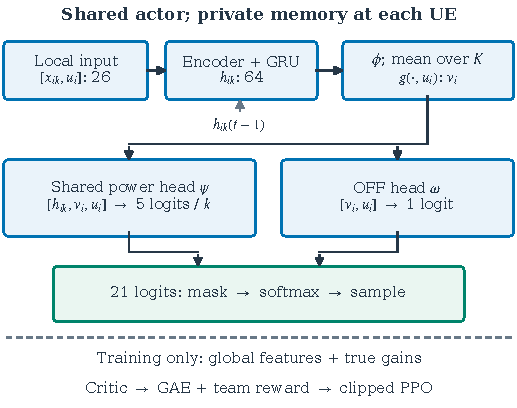
\includegraphics[width=\textwidth]{figures/mappo_framework.pdf}
\caption{Recurrent MAPPO architecture. Each UE runs the same actor with
private recurrent states, one per subchannel; the encoder, GRU, and channel
head share weights over $k$. Blue routing supplies the local context $u_i$;
both action heads also receive it. The delay $z^{-1}$ retains hidden state
across slots. The critic and global training inputs are absent at execution.
MAPPO-D adds the local multiplier to the context; MAPPO-F keeps that entry zero.}
\label{fig:framework}
\end{figure*}
\subsection{Shared recurrent actor}
Figure~\ref{fig:framework} shows the actor and centralized training pathway.
All devices share one actor but maintain private recurrent states. Its
subchannel tokens contain delayed RSSI, inferred interference, indicators of
the device's preceding transmission and power level, and estimated achievable
service at each power divided by required service $s_i/D_i$. The context
contains normalized remaining bits and time, the period, previous outcome and
service, and the remembered gain with a validity indicator. Logarithmic scaling
and clipping are applied to the rate ratios and physical quantities.

A shared encoder and gated recurrent unit (GRU) process each subchannel token
$x_{ik}(t)$ together with device context $u_i(t)$:
\begin{align}
h_{ik}(t)&=\operatorname{GRU}_{\theta}
  (f_\theta(x_{ik}(t),u_i(t)),h_{ik}(t-1)),\\
v_i(t)&=g_\theta\!\left(K^{-1}\sum_k\phi_\theta(h_{ik}(t)),u_i(t)\right).
\end{align}
A shared head maps $(h_{ik},v_i,u_i)$ to the power logits for subchannel $k$;
a separate head maps $(v_i,u_i)$ to the silence logit. A softmax over the
$1+K|\mathcal P|$ outputs defines $\pi_\theta$. This set aggregation follows
the permutation-invariant construction of Deep Sets~\cite{zaheer2017};
permuting the subchannel histories permutes their action logits. The GRU
state is updated during idle slots and retained across packet boundaries,
then reset when a new training or evaluation episode begins. Empty devices
are masked to $\OFF$.

\subsection{Training surrogate and constraint variants}
A centralized state-value critic observes all devices' features and true
gains during training. Let $c_i(t)$ be the deadline-violation indicator
settled at the end of slot $t$. The common training reward is
\begin{equation}
r_t=-\frac{1}{N}\left(\sum_i\frac{e_i(t)}{E_{\rm ref}}
                      +\sum_i\lambda_i(t)c_i(t)\right),\quad
E_{\rm ref}=\tau p_{\max}.\label{eq:reward}
\end{equation}
Our primary method, \emph{MAPPO-F}, sets $\lambda_i=w=10$ for all devices.
This fixed penalty is selected on validation data; it is a surrogate for the
per-device constrained problem, not an exact constrained solver.

The comparison method, \emph{MAPPO-D}, maintains a multiplier locally at each
device. At each of that device's deadlines,
\begin{equation}
\lambda_i\leftarrow\clip\bigl(\lambda_i+\eta(c_i-\epsilon),0,
                                  \lambda_{\max}\bigr).\label{eq:dual}
\end{equation}
The multiplier is also an actor input. We use $\eta=2$ and
$\lambda_{\max}=50$, independent uniform initial multipliers on $[0,50]$
during training, and a common
initial value selected from $\{0,5,25\}$ during validation. Execution updates
depend only on local outcomes. This is an application of state augmentation
with dual dynamics~\cite{calvo2021}, with no claim of a new dual algorithm
or inherited convergence guarantee under function approximation.

Both variants use recurrent MAPPO with a common generalized advantage estimate
from the centralized critic. For ratio
$\rho_{it}=\pi_\theta(a_i(t)\mid h_i(t))/
\pi_{\theta_{\rm old}}(a_i(t)\mid h_i(t))$, the actor maximizes
\begin{equation}
\E\!\left[\min\{\rho_{it}\widehat A_t,
       \clip(\rho_{it},1-\delta,1+\delta)\widehat A_t\}
       +\beta\mathcal H(\pi_\theta)\right].
\end{equation}
Only devices with pending packets contribute to the policy loss and entropy;
the critic learns from all slots. Ordered trajectory replay preserves recurrent
state. Technical episode truncations bootstrap the critic rather than marking
the continuing communication task terminal.

\section{Experimental Evaluation}\label{sec:experiments}
\subsection{Scenario, baselines, and protocol}
Table~\ref{tab:parameters} gives the common scenario and training parameters.
Device positions are sampled uniformly by area in a disk; gains are
$g_i=10^{-4}\max(d_i/1\,\mathrm{m},1)^{-4}$. Positions and phases remain fixed
within an episode. The three traffic classes have equal offered load per
device, so increasing $N$ raises load without changing its per-device average.
The class counts for $N=4,6,8,12$ are respectively $(2,1,1)$, $(2,2,2)$,
$(3,3,2)$, and $(4,4,4)$.

\begin{table}[t]
\caption{Scenario and learning parameters.}\label{tab:parameters}
\centering\footnotesize
\begin{tabular}{ll}
\toprule
Parameter & Value \\
\midrule
Devices / subchannels & $N\in\{4,6,8,12\}$ / $K=4$ \\
Slot duration / bandwidth & 1 ms / 1 MHz per subchannel \\
Cell radius / path-loss exponent & 100 m / 4 \\
Noise density / noise figure & $-174$ dBm/Hz / 7 dB \\
Positive transmit powers & 5, 10, 15, 19, 23 dBm \\
Periods $P_i$ (slots) & 10, 20, 40 \\
Packet sizes $L_i$ (bits) & 6144, 12\,288, 24\,576 \\
Per-device violation allowance & $\epsilon=0.05$ \\
Evaluation horizon / warm-up & 2000 / 200 slots \\
Training episode / rollout & 600 / 128 slots \\
Parallel environments / epochs & 16 / 4 PPO epochs \\
Actor GRU / critic hidden widths & 64 / 256, 256 \\
Actor / critic learning rates & $3\!\times\!10^{-4}$ / $10^{-3}$ \\
Discount / GAE parameter & 0.99 / 0.95 \\
PPO clip / gradient norm limit & 0.2 / 0.5 \\
Training budget per seed & $20\!\times\!10^6$ environment slots \\
\bottomrule
\end{tabular}
\end{table}

We train a separate shared policy for each $N$, using seeds 101, 202, and 303.
Each episode draws a topology--phase instance uniformly from a pool of one
million training instances. Training, development, validation, and test pools
are disjoint. Actor and critic parameters are not shared across network sizes;
the study tests generalization to new instances at a trained $N$, rather than
zero-shot transfer to a new $N$. The entropy coefficient decreases linearly
from 0.01 to zero over the first ten million slots. Total training slots are
summed over the 16 environments. Minibatches contain four environment
trajectories. The penalty and dual step size were selected in an initial
two-million-slot study at $N=8$ and transferred to all long runs.

Four local rules provide non-learning comparisons. \emph{Random-max} selects
a random subchannel and maximum power whenever a packet is pending.
\emph{Sticky-max} retains its preceding subchannel if its previous service
meets the current required pace, and otherwise reselects randomly, always at
maximum power. \emph{Lazy-pacing} selects power from its latest link estimate
to meet $s_i/D_i$, changing subchannel when necessary.
The strongest evaluated feasible rule, \emph{paced-sticky}, remembers its
gain across packets, retains a subchannel within 3 dB of the least-interfered
one, and otherwise switches with probability 0.5 to a subchannel within
3 dB of the minimum. It chooses the lowest power predicted to serve
$(1+m)s_i/D_i$ bits, probing at maximum power before its gain is known.
Its margin $m$ is calibrated over
$\{0,0.1,0.25,0.5,1,2,4,8,16,32\}$ separately for each $N$, selecting
$0,0.25,0.5,8$, respectively. Thus it is an energy-aware, load-calibrated
comparison rather than only a maximum-power random-access rule.

Validation uses 64 instances and one stochastic execution per instance,
approximately every million training slots. An episode is feasible if every
device has empirical violation rate at most 0.05. With $M_i$ evaluated
packets and $V_i$ violations, this is exactly
$V_i\le\lfloor0.05M_i\rfloor$ for all $i$. We denote the fraction of
feasible episodes by $F$. Among checkpoints with validation $F\ge0.95$, we
select the smallest mean normalized energy; if none qualifies, we select
the highest $F$, breaking ties by energy. MAPPO-D jointly selects its
initial multiplier. The selected and final checkpoints are both evaluated.

Testing uses 200 held-out instances per $N$, two executions per instance,
and all three training seeds. Random execution uses independent private
device streams with common seed assignments across methods. Evaluated packets
have deadlines in $(200,2000]$; their complete transmit energy, including
energy spent on failed packets, defines $E$. This packet-set accounting matches
the centralized denominators. Separately, reported mean power counts all
transmissions in slots $[200,2000)$. Methods satisfy the empirical protocol
criterion when their aggregate $F\ge0.95$. This threshold uses the point
estimate, not the lower confidence limit. Energy superiority is judged only
between methods satisfying it. We use 10\,000 two-level bootstrap resamples
over training seeds and instances, averaging repetitions within an instance.
Differences resample instances jointly and training seeds independently
between methods. All intervals are 95\% percentile intervals.

\subsection{Held-out energy and reliability}
\begin{figure*}[t]
\centering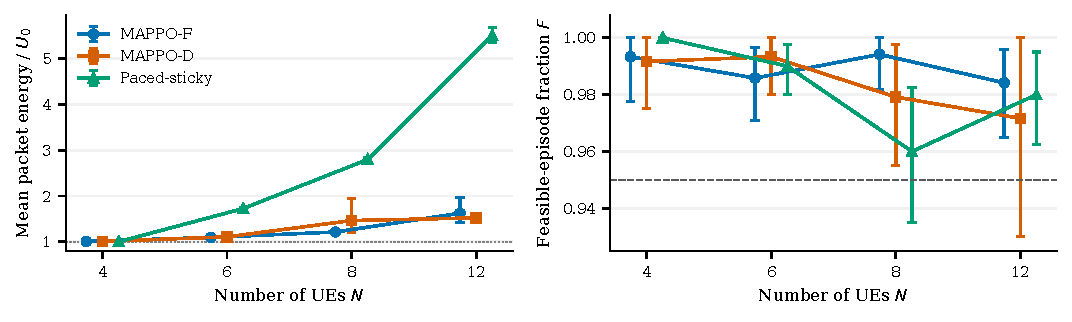
\includegraphics[width=\textwidth]{figures/test_performance.pdf}
\caption{Held-out test performance of selected checkpoints. The energy
denominator $U_0$ is a feasible centralized zero-loss schedule; it equals
the zero-loss optimum for $N=4$. Bars show two-level 95\% bootstrap intervals.
The dashed line at $F=0.95$ is the empirical protocol threshold.}
\label{fig:test}
\end{figure*}

\begin{table}[t]
\caption{All distributed methods on the held-out test set. Each cell is
$F$ / mean $E/U_0$. $\dagger$ denotes failure of the $F\ge0.95$ criterion;
its energy is descriptive only.}
\label{tab:all}
\centering\scriptsize\setlength{\tabcolsep}{2.2pt}
\begin{tabular}{lcccc}
\toprule
Method & $N=4$ & $N=6$ & $N=8$ & $N=12$ \\
\midrule
MAPPO-F & 0.993/1.01 & 0.986/1.09 & 0.994/1.21 & 0.984/1.62 \\
MAPPO-D & 0.992/1.01 & 0.993/1.11 & 0.979/1.46 & 0.972/1.52 \\
Paced-sticky & 1.000/1.00 & 0.990/1.73 & 0.960/2.80 & 0.980/5.51 \\
Random-max & 1.000/9.87 & 1.000/9.32 & 1.000/9.34 & 0.995/8.93 \\
Sticky-max & 1.000/10.36 & 1.000/10.05 & 1.000/10.40 & 0.983/10.21 \\
Lazy-pacing & 0.797/5.34$^\dagger$ & 0.657/4.98$^\dagger$ & 0.287/5.76$^\dagger$ & 0.000/8.02$^\dagger$ \\
\bottomrule
\end{tabular}

\end{table}

Figure~\ref{fig:test} and Table~\ref{tab:all} show that MAPPO-F satisfies the
empirical feasibility criterion at all four loads. For $N=6,8,12$, its mean
$E/U_0$ is \EnergySix, \EnergyEight, and \EnergyTwelve, compared with
1.725, 2.798, and 5.508 for paced-sticky. The reductions are
\SavingSix\%, \SavingEight\%, and \SavingTwelve\%, computed as one minus
the ratio of the two methods' mean normalized energies. They are not means
of per-instance percentage reductions. The paired differences
(MAPPO-F minus paced-sticky) have intervals
$[-0.659,-0.603]$, $[-1.632,-1.541]$, and $[-4.179,-3.535]$, respectively;
all exclude zero. Corresponding mean transmit powers are
\PowerSix, \PowerEight, and \PowerTwelve\,mW/device, versus
6.83, 12.07, and 29.24\,mW/device for paced-sticky.

At $N=4$, paced-sticky attains the exact zero-loss reference. MAPPO-F has
$E/U_0=1.007$ with interval $[1.004,1.010]$, and $F=0.993$.
This is a useful reference-recovery check, with no improvement over the local
rule at this load. At higher loads the learned policy's advantage over the
local rules grows, yet its distance from centralized scheduling also grows.
MAPPO-F's mean $E/L_0$ is 1.119, 1.349, and 2.289 for $N=6,8,12$.
At $N=12$, energy remains 62.3\% above the feasible orthogonal reference.
These ratios show substantial remaining room for improvement, with the
zero-loss qualification of Section~\ref{sec:bounds}.

Maximum-power rules retain high feasibility but consume approximately
9--10 times the centralized reference energy. Lazy-pacing fails the
feasibility criterion at every load, reaching $F=0$ at $N=12$.
Thus lowering power using only a recent pacing estimate does not by itself
resolve multiuser interference. The calibrated paced-sticky rule is
substantially stronger and remains the main energy comparison.

\subsection{Does local dual adaptation improve performance?}
Both selected MAPPO variants satisfy the empirical criterion at every $N$.
However, the paired energy difference between MAPPO-F and MAPPO-D has a
95\% interval containing zero at every load. At $N=8$, their means are
1.213 and 1.463, but the difference interval is $[-0.737,0.005]$;
at $N=12$, the means are 1.623 and 1.522, with interval
$[-0.119,0.452]$. One less effective training seed strongly affects each
comparison. These results give no statistically resolved energy advantage
to either constraint treatment; they do not establish equivalence.

Checkpoint dependence provides a practical distinction. MAPPO-F's final
checkpoints remain feasible at all four loads, with $F$ between 0.987 and
0.992. MAPPO-D's final $F$ falls to 0.915 and 0.938 at $N=8$ and 12.
The fixed-penalty variant therefore provides the simpler empirical reference
for this study. A separate short-budget global-multiplier variant selected
its untrained initial checkpoint and achieved test $F=0.592$ at $N=8$.
That result concerns this training configuration and selection outcome;
it does not show that global primal--dual methods generally fail.

\subsection{Training and observed coordination}
\begin{figure*}[t]
\centering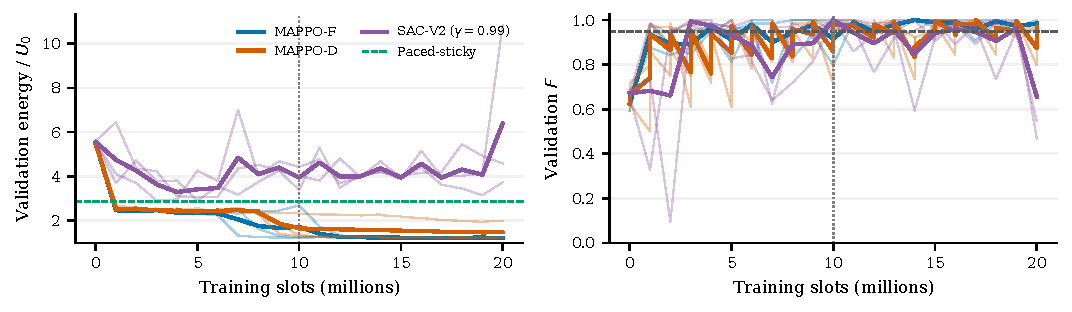
\includegraphics[width=\textwidth]{figures/learning_n8.pdf}
\caption{Validation trajectories for $N=8$. Thin lines show the three
training seeds; thick lines show their means, without smoothing. The vertical
dotted line marks the end of entropy annealing at ten million slots. For
MAPPO-D, curves use the validation-selected initialization at each checkpoint.
These are training diagnostics, not additional test-set evaluations.}
\label{fig:learning}
\end{figure*}

The gain requires substantial training. Figure~\ref{fig:learning} shows a
large energy decrease between roughly six and twelve million slots.
The separately trained two-million-slot MAPPO-F configuration has test
$E/U_0=2.321$ and $F=0.989$ at $N=8$; the long configuration reaches 1.213
and 0.994. Budget and entropy schedule both change between these configurations,
so the difference cannot be attributed to either change alone.

\begin{figure}[t]
\centering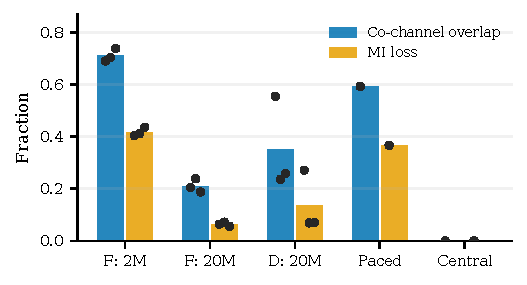
\includegraphics[width=\columnwidth]{figures/coordination_n8.pdf}
\caption{Descriptive validation diagnostics at $N=8$: short (2M) and long
(20M) training configurations. F and D denote MAPPO-F and MAPPO-D.
Bars are means across seeds; dots are individual seed summaries. The
central reference and paced-sticky have one summary each.}
\label{fig:coordination}
\end{figure}

To examine behavior, we replay selected policies on the validation set.
Co-channel overlap is the fraction of transmissions sharing their subchannel
with another active device; it does not mean automatic packet loss in the
SINR model. Interference loss is one minus the ratio of total actual mutual
information to the interference-free mutual information of those same
transmissions at the same powers. For MAPPO-F, the short-budget configuration
has mean overlap 0.712 and loss 0.418; the long configuration reduces these
to approximately 0.211 and 0.064 (Fig.~\ref{fig:coordination}).
Paced-sticky has overlap 0.594 and loss 0.367. Long-trained MAPPO-F also
uses the 5 and 10 dBm levels for about 83\% of transmissions.
Its probability of transmitting conditional on having a pending packet
is 0.61--0.76 across seeds, versus 1 for paced-sticky, consistent with using
silence while work is pending. This conditional fraction is not the fraction
of all device--slots that are occupied.

Together these observations support an association between energy savings,
lower-power transmission, and less harmful overlap. They do not isolate the
causal contributions of recurrence, power adaptation, or silence. A separate
validation-only short-budget experiment appended interference and own-action
features at lags of 10, 20, and 40 slots. It changed MAPPO-F's mean $E/U_0$
from 2.337 to 2.432, and MAPPO-D's from 2.404 to 2.385; neither met the
predeclared 5\% improvement threshold. This negative result is limited to
the tested features and budget, not all ways of exploiting periodicity.

\subsection{Reliability tails and scope}
The aggregate feasibility criterion allows a small set of bad episodes.
In a post hoc analysis pooling both learned variants over all four loads,
128 of 9600 executions are infeasible. In 108 of these, the worst device is
75--100 m from the AP, and in 83 its period is 40 slots. Such a device has
45 evaluated packets and can miss only two before the episode becomes
infeasible. Some failures are severe: an $N=4$ MAPPO-F execution contains
a device violation rate of 0.733. Average feasibility must therefore not be
read as a uniform reliability guarantee or a URLLC claim.

Three training seeds limit precision about optimization variability, and
the tested channel and feedback are idealized. Accounting for feedback,
circuit, and processing energy could change the benefit of spreading
transmissions. Further, this completed evaluation contains no independently
implemented literature-based learning comparator; it establishes an advantage
over the evaluated local rules. An information-matched XR-SBPC-style SAC
comparison is outside the completed evidence reported here.

\section{Conclusion}
A shared recurrent MAPPO controller learns energy-efficient uplink access
from local packet state and delayed AP feedback. With 6--12 devices sharing
four subchannels, MAPPO-F reduces mean normalized transmit energy by
\SavingSix\%--\SavingTwelve\% relative to calibrated paced-sticky access,
while meeting the per-device feasibility criterion. On the independent
eight-device confirmation set, the reduction reaches \ConfirmSavingSac\%
against an XR-SBPC-style SAC adaptation with the same energy reward and
execution information. Centralized zero-loss references quantify the
remaining energy gap. The learned policies combine low-power transmission
and selective silence with substantially reduced co-channel interference.


\bibliographystyle{IEEEtran}
\bibliography{references}
\end{document}
